\chapter{Introduction}
\hrule
\vspace{.5cm}



%%Contradiction section _________________________________%%
\section{Internet of Vehicles}
{
In the realm of the Internet of Vehicles (IoV), the convergence of advanced communication technologies and automotive systems has introduced a plethora of cyber attack vulnerabilities. IoV ecosystems, comprising interconnected vehicles, infrastructure, and backend services, are particularly susceptible to cyber threats due to their inherent complexity and reliance on networked communication. Attack vectors in IoV encompass a wide spectrum of malicious activities, ranging from remote vehicle hijacking and tampering with critical systems to theft of sensitive data and disruption of vehicular communication networks. With vehicles becoming increasingly connected and autonomous, the attack surface expands, providing adversaries with more opportunities to exploit vulnerabilities in software, hardware, and communication protocols. Furthermore, the integration of third-party services and aftermarket devices further exacerbates the security risks, as they may introduce additional entry points for cyber attacks. 

The distributed and dynamic nature of IoV environments also poses challenges for intrusion detection and response, as traditional security mechanisms designed for centralized systems may prove inadequate in this context. As such, safeguarding IoV ecosystems against cyber threats requires a multi-faceted approach, encompassing robust security protocols, threat intelligence sharing, continuous monitoring, and proactive mitigation strategies to ensure the safety, privacy, and integrity of connected vehicles and their occupants.

\begin{figure}[htbp]
\centerline{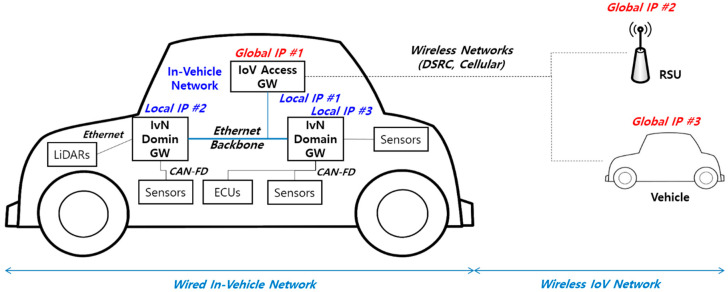
\includegraphics[width=0.7 \textwidth]
{img/iov_f.jpg}}
\caption{Internet of Vehicles architecture}
\label{fig}
\end{figure}

\par As modern vehicles become more connected and complex, their security is increasingly at risk. Cyber threats have the potential to compromise the stability and reliability of the Internet of Vehicles (IoV), leading to vehicle unavailability or even cause fatal traffic accidents.

\subsection{Cyber-Threats}
{

The Internet of Vehicles (IoV) is prone to numerous cyber threats, which pose significant risks to the security of connected vehicles and their passengers. Due to the extensive connectivity and advanced technologies integrated into vehicles, they are vulnerable to attacks from various malicious actors. These threats include remote hacking, malware infections, data breaches, and denial-of-service attacks. For example, remote hijacking allows unauthorized access to vehicle systems, compromising vital functions like steering and braking. Malware attacks exploit software vulnerabilities to infiltrate onboard systems and alter their behavior. Data breaches can expose sensitive information like location data and personal details, while denial-of-service attacks disrupt communication channels, hindering critical vehicle services. 

The compromised Electronic Control Units (ECUs) of internet of vehicles may be exploited by malicious actors to engage in such types of attacks. For instance, a real demonstration of car hacking illustrated in \cite{miller2015remote} revealed the vulnerability of a Jeep Cherokee to be compromised and stopped remotely while driving on a highway.

Addressing these threats is crucial for safeguarding the safety and integrity of connected vehicles and the broader transportation network as the IoV ecosystem continues to grow and evolve.


% remote compromise, resulting in the ability to halt the vehicle while it was in motion on a highway.
}

}


\section{Intrusion Detection Problem}
{
Intrusion detection is a crucial component in modern Internet of Vehicles to recognize harmful attacks on automotive networks. It is still a hard problem in IoV because of a vast amount of network traffic data, a variety of network properties, and numerous cyber-attack methods.

}

\section{Objectives}
\begin{itemize}
\item To successfully detect recognized cyber-attacks on both intra-vehicular and external vehicular networks by applying various machine learning algorithms.
\item To evaluate the performance and overall effectiveness of
the proposed model on two labelled datasets, CAN-intrusion dataset and the CICIDS2017 dataset.

\end{itemize} 
